\pagestyle{fancyplain}

\label{lab:chapPET}
La Tomographie par \'Emission de Positons (TEP) au fluoro-deoxy-glucose marqué au Fluor 18 ($^{18}$FDG) est une modalité d'imagerie fonctionnelle utilisant la désintégration d'un traceur radioactif pour mettre en valeur les zones de forte activité métabolique. Elle est principalement utilisée en imagerie cérébrale, oncologique et cardiologique.


Dans ces trois chapitres, nous allons tout d'abord détailler rapidement les principes physiques amenant à la création des images TEP, de la désintégration du traceur radioactif à la détection des photons émis lorsqu'ils atteignent un capteur. Ensuite, nous parlerons des solutions techniques mises en place pour réaliser les images TEP, avec les différents types d'acquisitions. Enfin, nous détaillerons les algorithmes utilisés pour reconstruire les images TEP.

 
\chapter{Principe Physique}

	\section{Généralités}

L'imagerie TEP est basée sur l'injection d'une molécule traceuse marquée par un atome radioactif émetteur de positon. Ce paragraphe présente rapidement les événements qui se produisent lors d'un examen TEP, présentés dans la figure~\ref{fig:schemaTEP}.

Ce traceur est conçu de manière à se fixer sur les zones du corps que l'on souhaite imager. Pendant toute la durée de l'examen, les particules radioactives vont se désintégrer selon la loi de décroissance radioactive de l'équation~\ref{eq:loidecradioact}.

\begin{equation}
	dN = - \lambda N dt
	\label{eq:loidecradioact}
\end{equation}

$N$ représente le nombre de particules radioactives présentes dans le corps du patient. $dN$ représente la variation de ce nombre de particules (le nombre de désintégrations par $dt$) et $\lambda$ est une constante dépendant de l'élément radioactif.

Chaque désintégration d'un élément radioactif va déclencher l'émission d'une particule chargée $\beta^+$, aussi appelée positon. En oncologie, on utilise par exemple le Fluor $^{18}F$ qui se désintègre en Oxygène $^{18}O$ en émettant un positon. Cette particule va parcourir quelques mm avant de s'annihiler avec un électron en émettant 2 photons dans deux directions opposées avec une énergie de 511 KeV.

Ce sont ces photons qui sont détectés par l'imageur TEP. Ils représentent une coïncidence, car l'instant d'arrivée et leur énergie sont approximativement semblables. L'ensemble des ``lignes de réponse'' (LDR) correspondant aux coïncidences détectées est utilisé pour reconstruire les images.

\begin{figure}
\centering
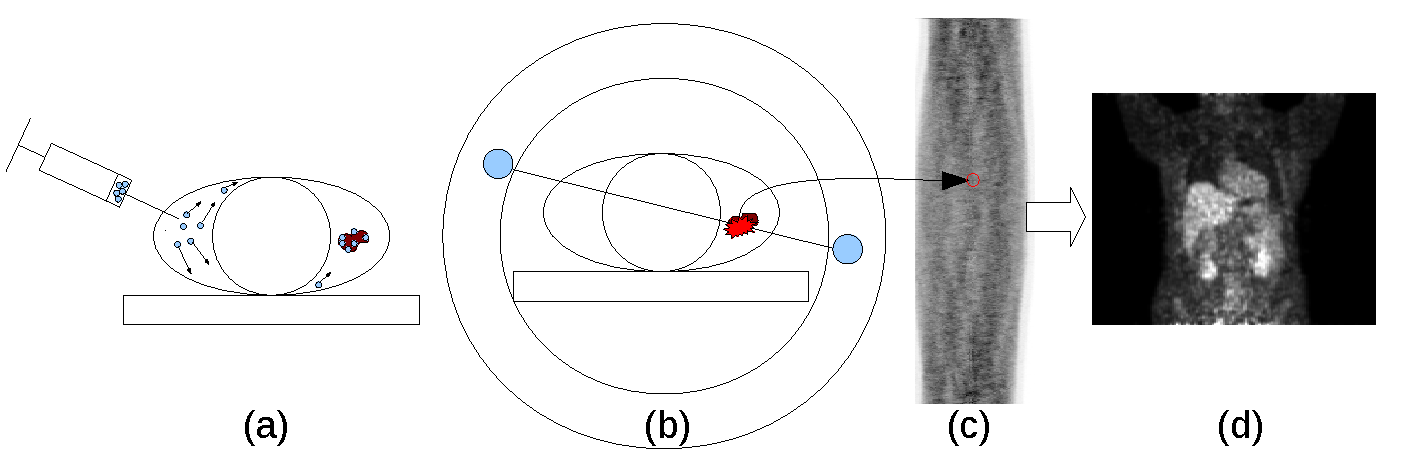
\includegraphics[width=16cm]{images/schemaTEP}
\caption[Présentation simplifiée de la TEP]{Processus d'un examen TEP : a) Injection du traceur radioactif, qui va se fixer préférentiellement sur les zones que l'on cherche à observer. b) Désintégration d'un atome radioactif du traceur, ici dans la zone à imager. Cela entraîne l'émission de deux photons dans deux directions opposées, qui sont détectés dans la couronne de capteurs. c) Tous les événements détectés sont stockés dans la mémoire de la console, ici sous forme de sinogramme. d) L'image est reconstruite à la suite de l'acquisition pour former un volume 3D estimant la répartition du traceur dans l'organisme.}
\label{fig:schemaTEP}
\end{figure}


\section{Traceur $^{18}$FDG}

Le glucose est considéré comme un carburant essentiel à l’organisme qui peut l’assimiler directement. Les cellules cancéreuses, qui ont un métabolisme accéléré par rapport aux autres cellules du milieu, sont particulièrement friandes de glucose. Celui-ci est transporté à l’intérieur des cellules par des transporteurs spécifiques de la membrane afin d’être dégradé par un ensemble de réactions appelé glycolyse. Le glucose est d’abord phosphorylé en glucose-6-phosphate, catalysé par l’enzyme hexokinase. Le glucose-6-phosphate est ensuite transformé en fructose-6-phosphate qui subit à son tour plusieurs transformations successives pour être finalement excrété par la cellule sous forme de lactate.

Le fluorodeoxyglucose ou FDG est un analogue du glucose avec un aspect structural très proche. Il est donc aussi capté par les cellules, mais ne peut pas être utilisé dans leur métabolisme. Le FDG suit le même processus métabolique que le glucose jusqu’à l’étape de phosphorylation en FDG-6-phosphate. Il n’est cependant pas métabolisé par l’enzyme glucose-6-phosphate et s’accumule dans la cellule sous la forme de FDG-6-phosphate. Cette accumulation permet de distinguer la présence de tumeurs, généralement beaucoup plus gourmandes en énergie que les tissus sains et donc marquées par une présence élevée de FDG-6-phosphate. Par son métabolisme et son importance pour les cellules cancéreuses, le FDG est actuellement préconisé en clinique pour les examens concernant des patients en cancérologie. Il est généralement marqué au fluor 18 donnant le $^{18}$FDG.

Cependant, ce radiotraceur n'est pas spécifique aux tumeurs mais se fixe sur toute cellule consommant du glucose. C'est pourquoi le coeur ainsi que le cerveau fixent toujours une grande quantité de $^{18}FDG$, comme l'indique la figure~\ref{fig:schemaTEP}.d).

\section{\'Emission des photons}

Nous allons maintenant détailler le processus qui déclenche l'émission des photons détectés par l'imageur, présenté dans la figure~\ref{fig:Langner2008ad}.

Les émetteurs de positons utilisés en TEP sont des isotopes radioactifs présentant un excès de charge positive, ou proton, dans leurs noyaux. Un processus de désintégration $\beta^+$, correspondant à la transformation d’un proton $p$ en un neutron $n$, leur permet de migrer vers un état stable. Cette désintégration résulte en l’émission d’un neutrino $\nu$ et d’un positon $e^+$ selon l’équation~\ref{eq:desinteg}. Le positon est une particule de même masse que l’électron mais de charge opposée.

\begin{equation}
 p~\rightarrow~n + e^+ + \nu
\label{eq:desinteg}
\end{equation}

Le positon va alors s'annihiler avec un électron après un parcours de quelques millimètres en émettant simultanément deux photons $\gamma$ de même énergie (511 keV), comme indiqué dans l'équation~\ref{eq:annihilation}. L'angle d'émission des photons $\gamma$ est de $180°$ avec une incertitude de $\pm 0.25°$~\cite{bailey2005positon}.

\begin{equation}
 e^+ + e^-~\rightarrow~\gamma + \gamma
\label{eq:annihilation}
\end{equation}

\begin{figure}
\centering
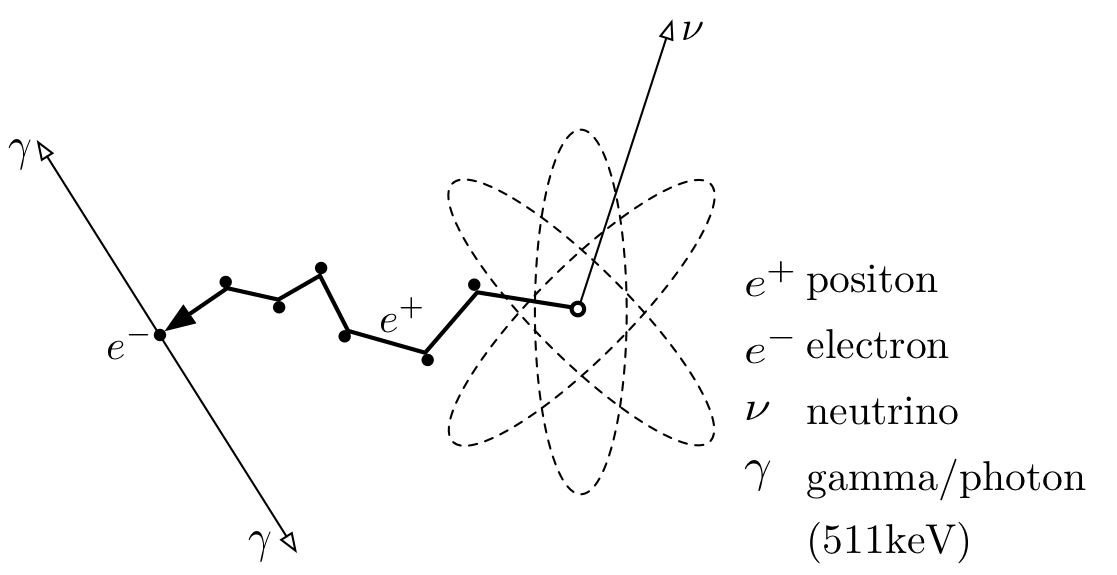
\includegraphics[width=12cm]{images/annihilation}
\caption[\'Emission des photons]{\'Emission des photons~\cite{Langner2008ad} : Le radio traceur se désintègre en émettant un neutrino et un positon. Après un parcours de quelques mm dans les tissus, ce dernier s'annihile avec un électron. Cette réaction provoque la création de deux photons $\gamma$ d'énergie 511 keV partant dans deux directions opposées.}
\label{fig:Langner2008ad}
\end{figure}

\section{Détection des photons}

Les détecteurs les plus couramment utilisés en TEP sont constitués d'un couplage entre un cristal scintillant et un tube photomultiplicateur.

Le cristal scintillant permet de convertir les photons $\gamma$ de 511 keV en photons lumineux par les différents phénomènes d'interaction particules-matières.

Chaque photon absorbé par le matériau scintillant va entraîner une réaction en chaîne qui va déclencher une émission lumineuse. Le tube multiplicateur situé derrière va convertir cette émission lumineuse en charge électrique. Un système électronique va ensuite apparier les photons détectés pour retrouver la ligne de réponse (LDR) sur laquelle la désintégration a eu lieu. Les paires de photons assemblées correspondent à des coïncidences.

Les détecteurs sont regroupés par modules, placés en anneaux autour du patient. L'imageur TEP Gemini que nous utiliserons dans cette étude dispose par exemple de 28 modules, contenant chacun une matrice de 29 par 22 cristaux de GSO (voir figure~\ref{fig:moduleTEP}). Une photo de l'imageur ouvert est visible sur la figure~\ref{fig:gemini_ecl}. 420 photomultiplicateurs placés autour des blocs sont utilisés pour estimer la position des détections.

\begin{figure}
\centering
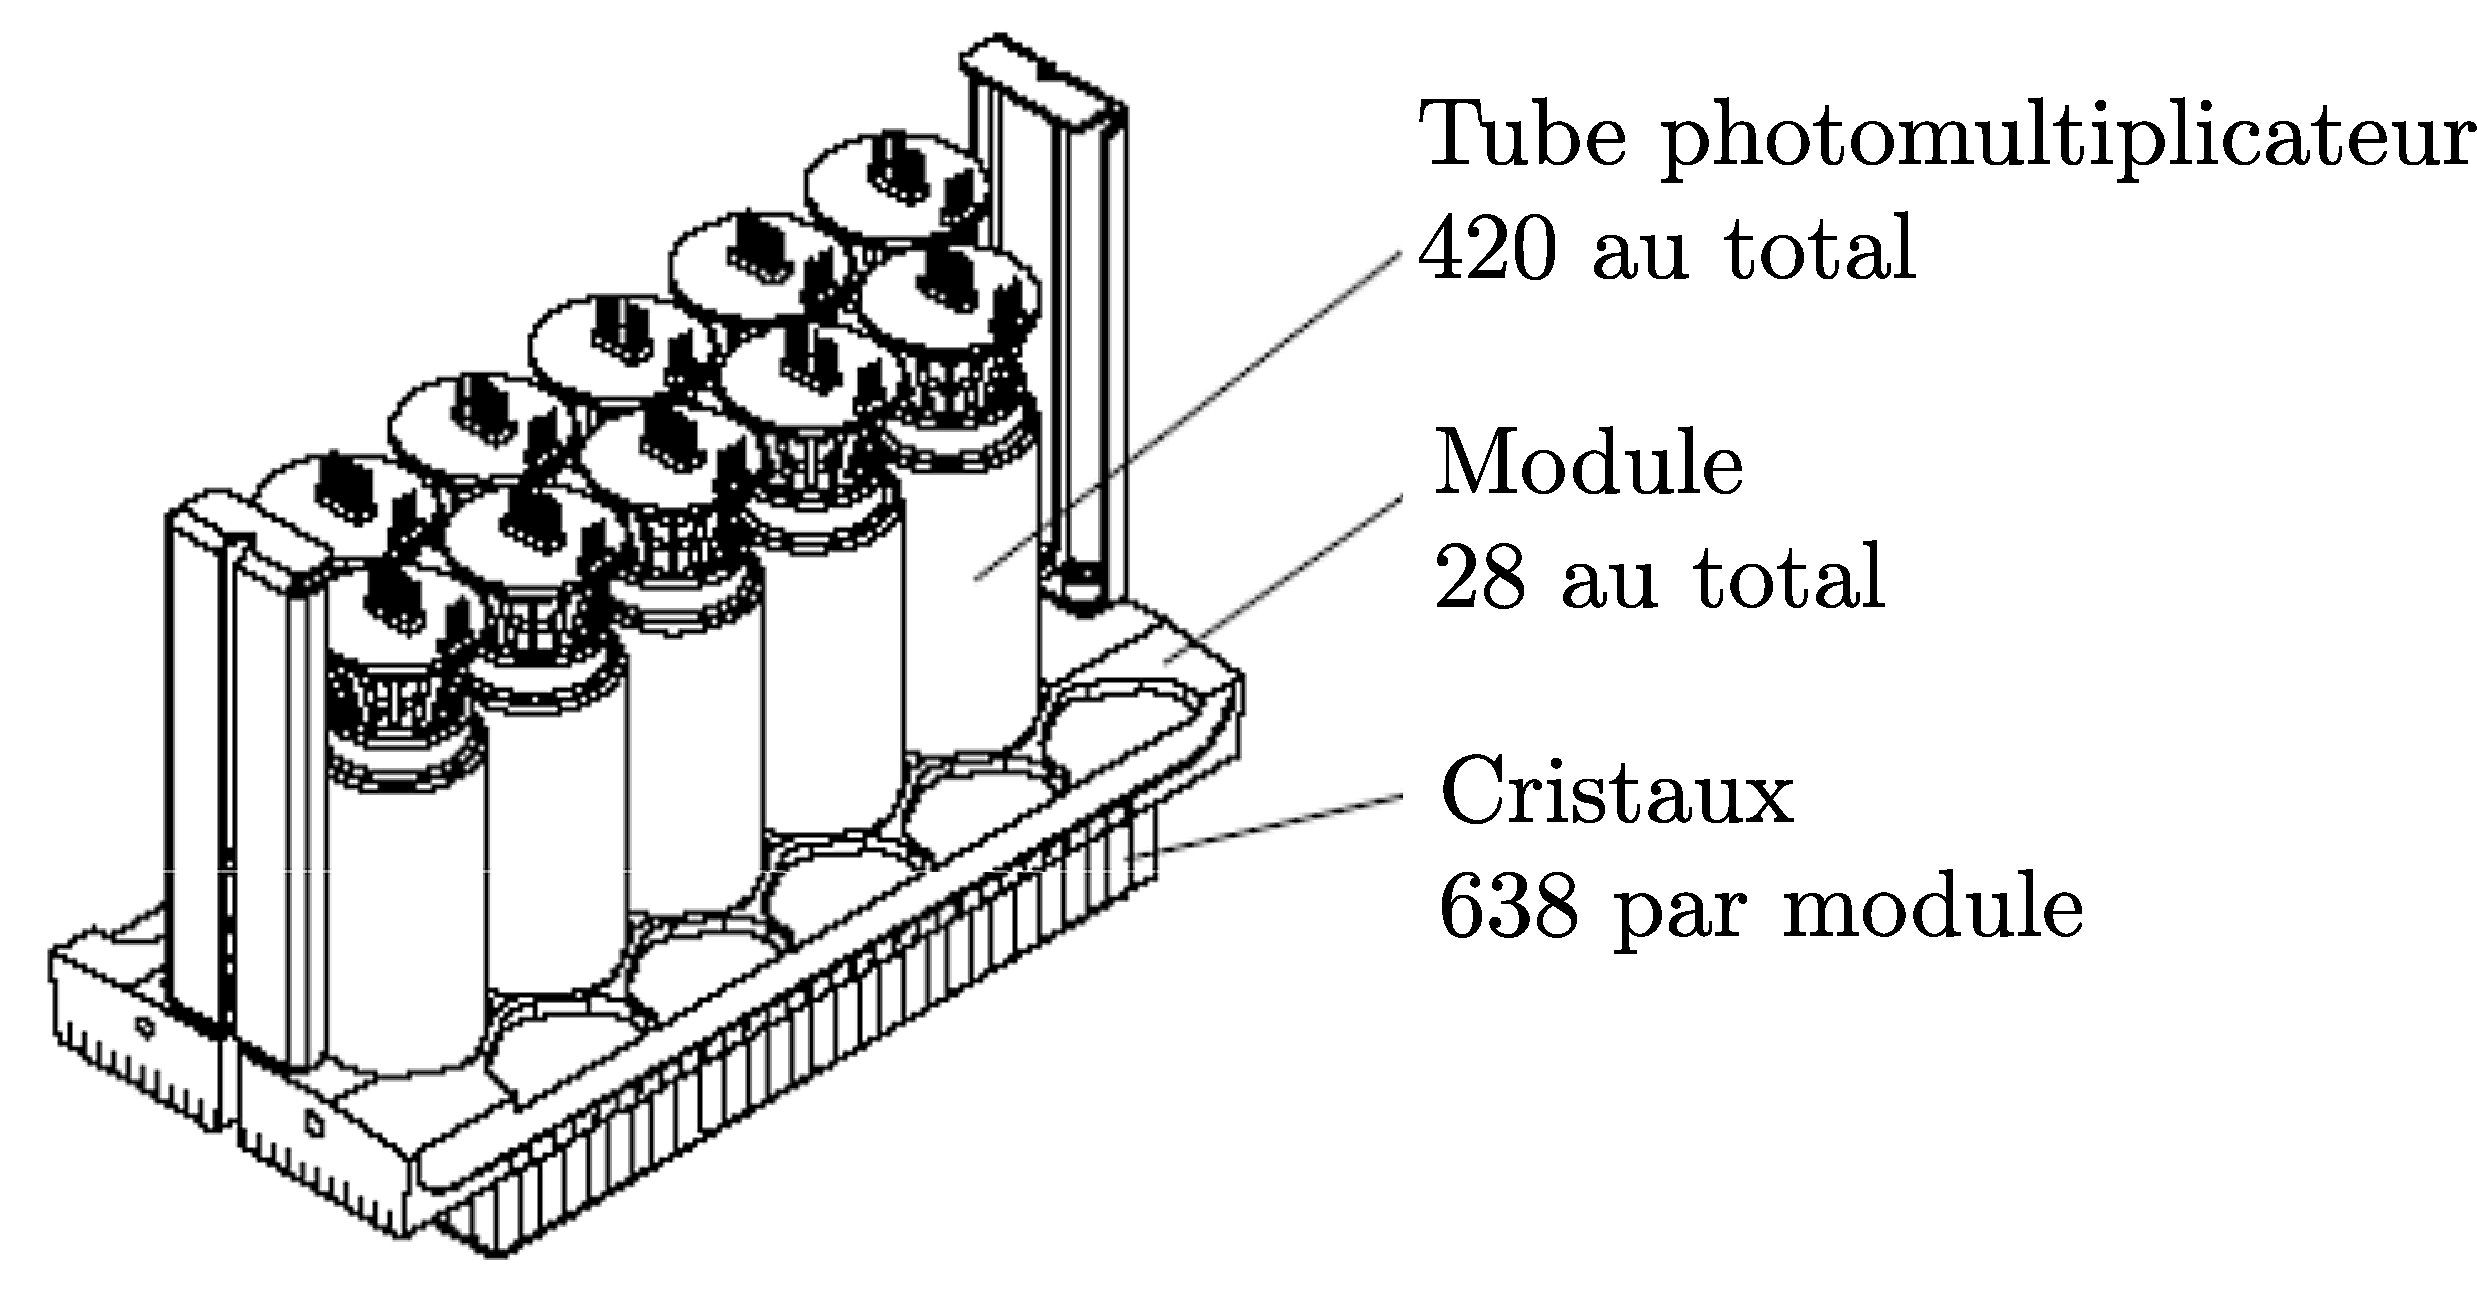
\includegraphics[width=8cm]{images/coupe_module}
\caption[Coupe d'un module de Philips Allegro]{Coupe d'un module de Philips Allegro. Les 28 modules sont placés en anneaux autour du patient.}
\label{fig:moduleTEP}
\end{figure}


\begin{figure}
\centering
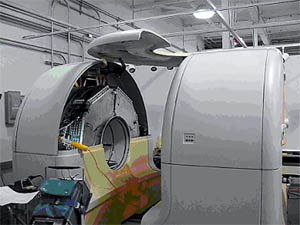
\includegraphics[width=12cm]{images/gemini_eclate}
\caption[Photo d'un imageur Philips Gemini ouvert]{Cette photo représente la partie PET d'un imageur Philips Gemini ouverte. On distingue les cartes électroniques connectées aux tubes photomultiplicateurs.}
\label{fig:gemini_ecl}
\end{figure}

	\section{Types de coïncidences}

La figure~\ref{fig:schemaDetections} représente les différents types de coïncidences rencontrés en TEP.

Les coïncidences vraies (\ref{fig:schemaDetections}.a) correspondent aux cas où les deux détections appariées correspondent bien à une seule désintégration et où aucun des photons n'a été dévié. Les coïncidences fortuites (\ref{fig:schemaDetections}.b) correspondent à la détection en coïncidence de deux photons issus de deux annihilations différentes, par exemple à cause de l’absorption d’un des photons d’une désintégration par les tissus. Enfin, les coïncidences diffusées (\ref{fig:schemaDetections}.c) sont le résultat de la déviation d'un des deux photons produit engendré par des interactions rayonnement-matière dans les tissus (diffusion Compton). 

%Pour éliminer ces erreurs, un certain nombre de méthodes ont été implémentées, dont le filtrage en énergie et en temps au niveau matériel : ne sont prises en compte que les paires d'événements arrivant dans une fenêtre temporelle et énergétique définie. En effet, les photons déviés vont perdre de l'énergie, ce qui va entraîner leur élimination.


Les coïncidences diffusées ainsi que les coïncidences aléatoires génèrent un bruit parasite dans les sinogrammes. L'absorption des photons sans détection va engendrer un effet d'atténuation du signal qui sera de plus en plus important en fonction de la profondeur des tissus et de leur absorption.


\begin{figure}
\centering
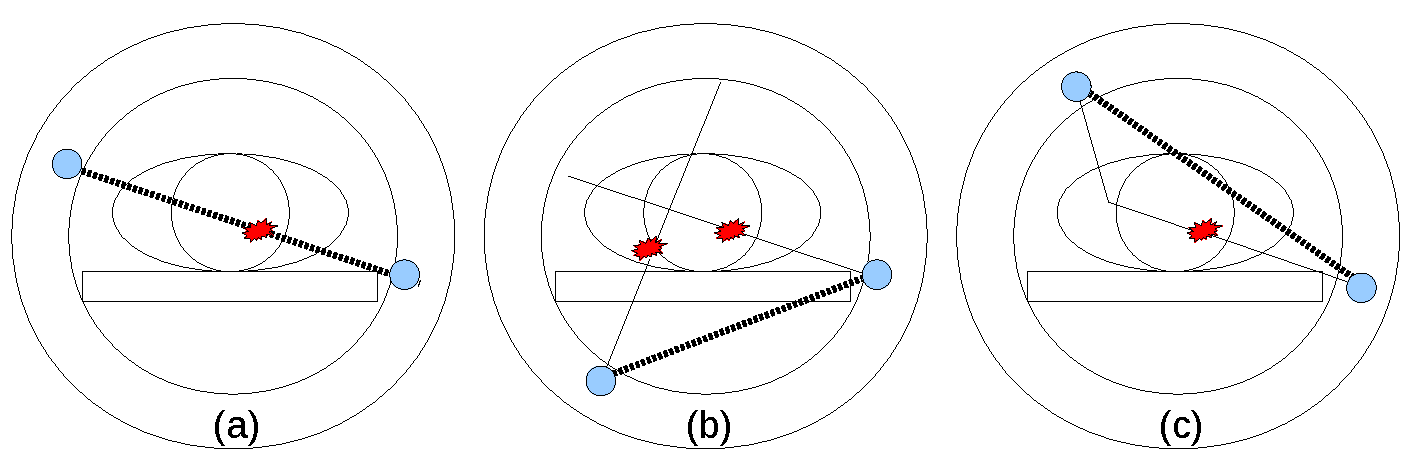
\includegraphics[width=12cm]{images/schemaDetections}
\caption[Les différents types de coïncidences en TEP]{Les différents types de coïncidences en TEP. Le trajet réel du photon est indiqué en trait fin simple, tandis que la ligne de réponse est indiquée en trait pointillé épais. On appelle les coïncidences vraies (a) lorsque l'annihilation est bien sur la ligne de réponse, fortuites (b) lorsque deux désintégrations réalisées en même temps sont considérées comme une seule et diffusée (c) lorsqu'un des photons est dévié.}
\label{fig:schemaDetections}
\end{figure}



	\section{Perturbation du trajet du photon}

Les deux interactions les plus importantes que peuvent avoir les photons avec les tissus sont la diffusion Compton et l'absorption photo-électrique~\cite{cherry2006pet}. L'effet Rayleigh, qui correspond à la diffusion du photon sur un atome, est peu présent aux énergies concernées par la TEP. 

La diffusion Compton correspond à l'interaction entre le photon émis et un électron du milieu. L'énergie cinétique de l'électron est augmentée, tandis que le photon est dévié. Il est intéressant de noter qu'une déviation de 25° engendre une perte d'énergie du photon de seulement 10\%~\cite{evans1955atomic}.

L'absorption photo-électrique correspond quant à elle à l'interaction entre un noyau atomique et un des photons. L'énergie du photon est absorbée par le noyau et transmis à un de ses électrons. 

L'atténuation du signal est liée à une combinaison de ces effets. L'effet d'atténuation est particulièrement important en TEP, car il génère des artefacts très visibles, qui doivent être corrigés à partir d'une carte d'atténuation, déduite d'un examen de tomodensitométrie (tomographie par rayons X) ou d'une carte de transmission, comme indiqué sur la figure~\ref{fig:schemaAtt}.


On peut représenter cette atténuation de manière analytique à l'aide de la loi de Beer-Lambert~\cite{cherry2006pet}, qui montre que l'atténuation augmente exponentiellement avec la longueur du trajet dans les tissus :
\begin{equation}
I = I_0 e^{-\mu l}
\end{equation}

Avec $I_0$ la quantité originale de photons, $I$ le nombre de photons qui traversent le milieu, $\mu$ le coefficient d'atténuation du milieu et $l$ la longueur du trajet. 

Dans le cas où le milieu est complexe, et si l'on connaît l'atténuation $\mu(x)$ en chaque point $x$ du trajet, on peut connaître précisément l'atténuation subie selon chaque ligne de réponse  :

\begin{equation}
I = I_0 e^{- \int\limits^L_0 \mu(l) dl}
\end{equation}


\begin{figure}
\centering
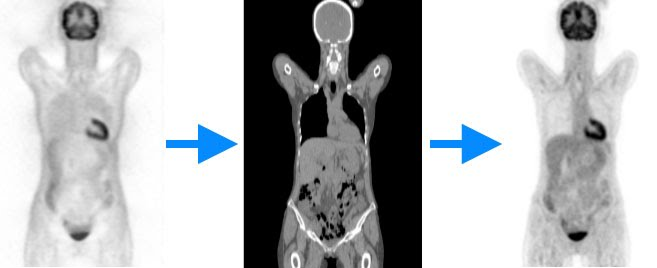
\includegraphics[width=12cm]{images/attenuationNonAtt}
\caption[Effet de l'atténuation sur les images TEP]{Effets de l'atténuation sur des images TEP : L'image de gauche correspond à la distribution de radioactivité reçue par les détecteurs. On peut observer une perte progressive de l'activité vers l'intérieur des tissus, car les photons ont plus de chances d'interagir avec la matière. L'image TDM au centre est utilisée pour estimer une carte de l'atténuation des tissus et prendre en compte cette atténuation lors de la reconstruction de l'image TEP.}
\label{fig:schemaAtt}
\end{figure}

\section{Quantification en imagerie TEP}

L'image visualisée par le clinicien est directement liée à  la concentration de l'isotope radioactif. La concentration observée est la somme de la concentration du traceur piégé dans les cellules et du traceur libre dans le compartiment vasculaire. Cette concentration mesurée est très dépendante du volume du patient, ainsi que de la dose injectée.

En clinique, on utilise habituellement le SUV (Standard Uptake Value), qui est un index semi-quantitatif permettant de s'affranchir de la dose injectée et des caractéristiques morphologiques du patient. Cela permet de réaliser des comparaisons entre des fixations radioactives de plusieurs examens, voire de plusieurs patients.

Le SUV est défini comme suit :

\begin{equation}
SUV=\frac{C}{ \frac{dose~inject\acute{e}e}{poids~corporel} }
\end{equation}

Où C est la concentration du traceur radioactif.

Des méthodes, plus complexes, basées sur des acquisitions dynamiques et la connaissance \textit{a priori} d'un modèle de distribution du traceur dans l'organisme, permettent de remonter à des paramètres biologiques, tels que la consommation de glucose par gramme de tissus et par unité de temps pour le FDG. Ces méthodes sont en pratique peu utilisées en routine clinique en raison de la difficulté et du coût de réalisation des acquisitions dynamiques.

\chapter{Déroulement d'une acquisition}


Nous allons maintenant décrire rapidement quelques points techniques permettant de mieux comprendre comment sont réalisées les acquisitions TEP en routine clinique. Nous parlerons de la méthode utilisée pour réaliser des acquisitions corps entier alors que l'imageur a un champ de vue axial limité et des contraintes associées. Enfin, nous aborderons la problématique du format des données et ses implications.

\section{TEP au $^{18}$FDG}


En oncologie, les patients qui ont une suspicion de cancer se voient proposer un examen TEP pour réaliser un diagnostic initial, qui va viser à déterminer le degré de malignité de la pathologie détectée. Il a été montré~\cite{gould2001accuracy} que les performances de la TEP sur la détection des lésions pulmonaires étaient supérieures à l'imagerie anatomique. Les performances de la TEP sont aussi reconnues pour les cancers hépatiques et la détection précoce des lymphomes. Plusieurs images sont visibles dans la figure~\ref{fig:exTEP}.

La TEP est ensuite utilisée pour suivre l'évolution des lésions, afin d'adapter le traitement à l'évolution de la maladie.

\begin{figure}[h!]
\centering
\begin{tabular}{c c c}
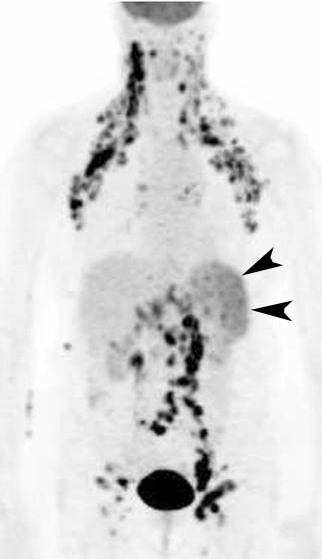
\includegraphics[width=5cm]{images/ex_lymphome} & 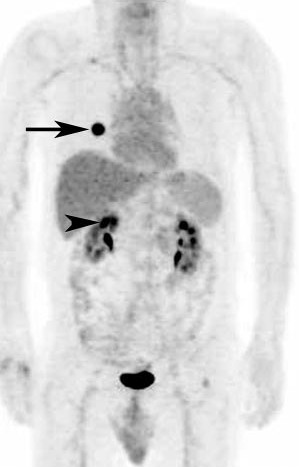
\includegraphics[width=5cm]{images/ex_poumon} & 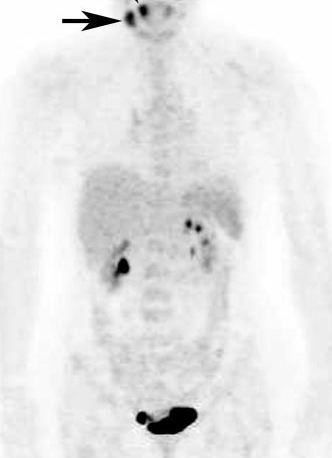
\includegraphics[width=5cm]{images/ex_cou} \\
a) & b) & c)
\end{tabular}
\caption[Exemples d'images TEP]{Exemples d’images TEP au $^{18}$FDG provenant d’examens de patients atteints d’un cancer a) des ganglions (lymphome), b) du poumon et c) du cou. Certaines lésions sont représentées par les flèches noires. Les image sont extraites de l'article~\cite{rohren2004clinical}.}
\label{fig:exTEP}
\end{figure}

\section{Acquisitions corps entier}


Les acquisitions TEP réalisées pour l'oncologie sont habituellement des acquisitions corps entier, de manière à pouvoir avoir une vue de l'étendue des lésions.

Or le champ de vue axial de la plupart des caméras TEP est de l'ordre de 15 à 20 cm environ (18 cm pour le Philips allegro~\cite{lamare2006validation}). En routine clinique, le patient est placé sur un lit qui se déplace par incréments successifs lors de l'acquisition. Une photographie de l'imageur avec le lit est présentée dans la figure~\ref{fig:photoGemini}.

\begin{figure}
\centering
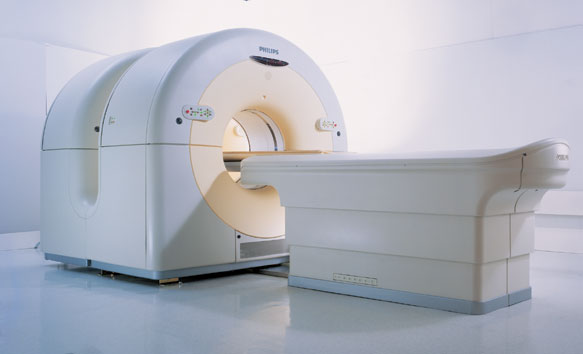
\includegraphics[width=12cm]{images/gemini}
\caption[Photographie d'un scanner TEP Gemini]{Photographie d'un scanner TEP/TDM Gemini. Le lit motorisé est présenté au premier plan et permet de faciliter le déplacement du patient au cours de l'acquisition.}
\label{fig:photoGemini}
\end{figure}

Le nombre de positions du lit est déterminé par la taille du patient ainsi que par le champ de vue du tomographe. Chaque lit est reconstruit séparément puis assemblé avec les lits suivants et précédents, comme indiqué dans la figure~\ref{fig:multilits}. \'Etant donné que les caméras TEP ont une sensibilité plus faible à leurs extrémités, on introduit un chevauchement plus ou moins important dans les lits.

\begin{figure}
\centering
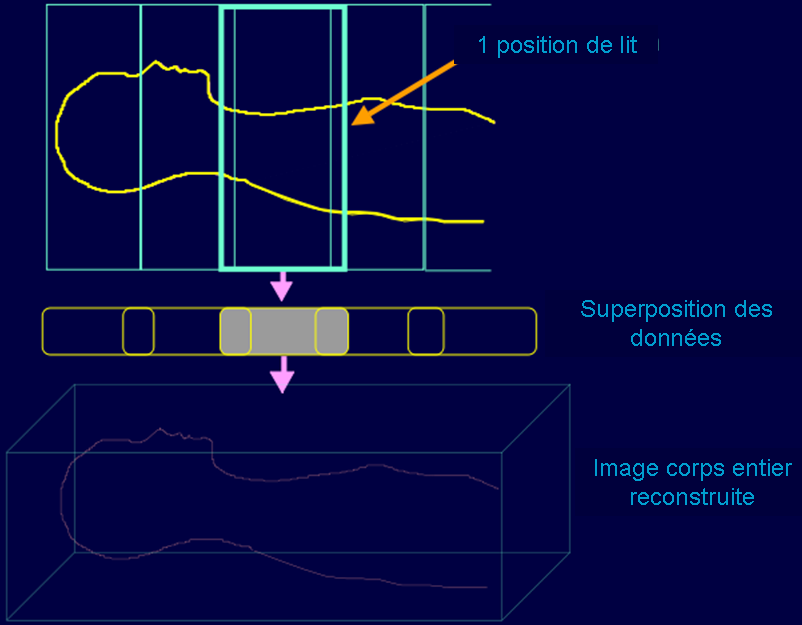
\includegraphics[width=10cm]{images/multilits}
\caption[Acquisitions corps entier en TEP]{Réalisation d'une acquisition corps entier en TEP : Chaque lit est acquis et reconstruit séparément avec un chevauchement. Les lits sont ensuite assemblés pour produire l'image finale.}
\label{fig:multilits}
\end{figure}

Les acquisitions corps entier utilisent typiquement plus de 10 lits sur la caméra Philips Gemini, ce qui demande un temps considérable. Il faut donc faire des compromis entre le temps d'acquisition et la qualité des images. Sachant que les examens TEP sont coûteux et que l'immobilité est inconfortable pour les patients, le temps d'acquisition est calibré pour durer moins d'une heure au total. Les nouvelles générations d'imageurs permettent cependant de réduire les temps d'acquisition à 2 minutes par lit à qualité équivalente.


	\section{Acquisition en mode 3D}

Historiquement, les données étaient acquises par coupe : des septas (plaque destinées à absorber les photons) étaient placés entre les détecteurs dans la direction axiale de manière à éliminer les photons qui n'étaient pas émis dans le plan  transverse (perpendiculaire à l'axe du détecteur). Aujourd'hui, la totalité des scanners fonctionnent en mode 3D uniquement. Le retrait des septa (voir la figure~\ref{fig:2D3D}) permet d'augmenter le rapport signal sur bruit pour les gammes d'activité injectées aux patients, même si la détection des coïncidences vraies s'accompagne d'une augmentation de bruit parasite liée à l'augmentation de la détection des coïncidences fortuites et diffusées.

\begin{figure}
\centering
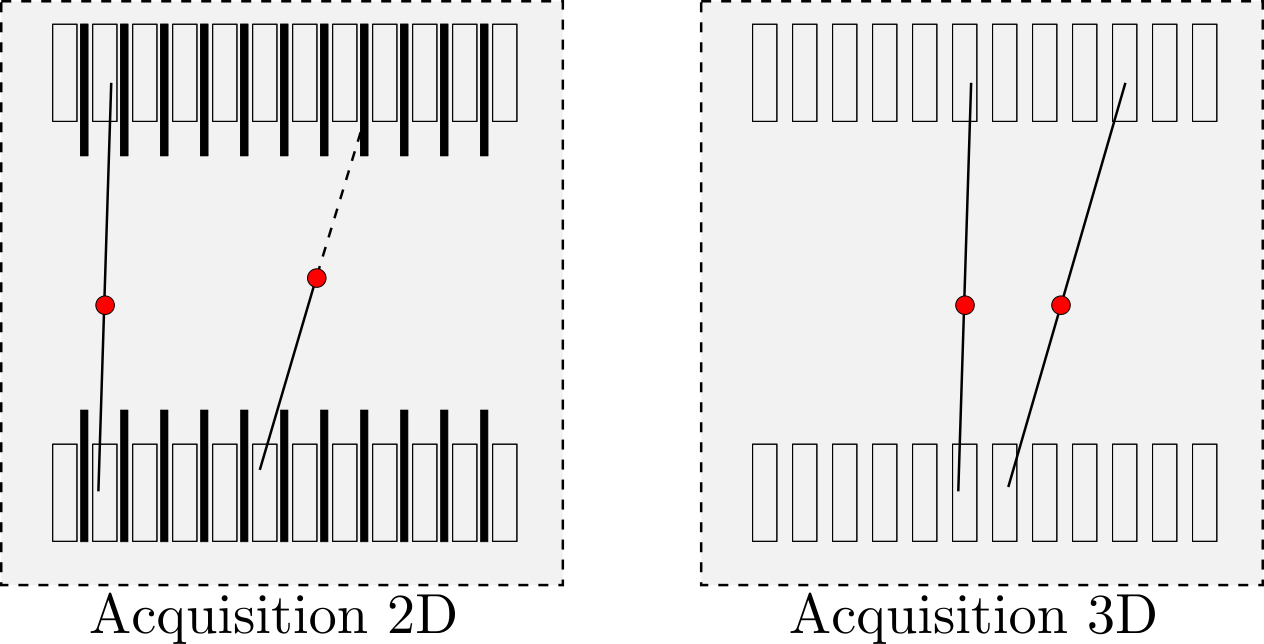
\includegraphics[width=6cm]{images/2D3D}
\caption[Acquisitions 3D en TEP]{Coupe schématique axiale d'un imageur TEP. Les annihilations représentées en rouge émettent des photons qui sont détectés par des cristaux correspondant à des plans de coupes différents.}
\label{fig:2D3D}
\end{figure}


%	\section{Corrections}

	\section{Correction de l'atténuation}
\label{CorrectionAttenuation}

Le patient passe tout d'abord un examen TDM sur les scanners couplés TEP/TDM. Les valeurs des coefficients Hounsfield correspondant à l'atténuation des rayons X sont transformées pour correspondre à l'atténuation des photons de 511keV de la TEP. Cette image est ensuite utilisée pour réaliser la correction d'atténuation. 

Une technique plus ancienne d'estimation de la carte d'atténuation est basée sur une image acquise en transmission, où une source radioactive émettrice de positons est placée dans l'imageur et tourne autour du patient. Une acquisition  préalable est réalisée ``à blanc'', sans le patient. Le rapport entre la quantité de photons reçue par les détecteurs avec et sans le patient permet de générer la carte d'atténuation du corps du patient, de la même manière que pour l'imagerie TDM. Cependant, la généralisation des scanners couplés TEP/TDM limite l'utilisation de cette technique.

\begin{equation}
I(x) = I_0(x) e^{-\mu x}
\end{equation}

En connaissant la radioactivité reçue sans le patient (``à blanc'') $I_0$, la radioactivité reçue avec le patient $I$, on peut en déduire la valeur de $\mu$.

%\subsection{Correction des coïncidences fortuites}

%Des techniques existent pour corriger les données des effets vus dans la figure~\ref{fig:schemaDetections}, notamment l'implantation d'une ligne à retard pour estimer les coïncidences aléatoires puis les retirer du sinogramme.

	\section{Correction des autres sources de bruit}

\subsubsection{Correction de temps mort}


Le temps mort correspond à l’intervalle de temps durant lequel le dispositif est insensible après le passage d’une impulsion électrique. Lorsque deux impulsions surviennent avec un décalage temporel inférieur au temps d’intégration, seule la première est traitée et la deuxième est perdue. La correction de ce temps mort consiste à modéliser les pertes de comptage en événements pour chaque module de détection. En effet, le taux de photons simples $s$ et le facteur de temps mort, noté $d_{tk}$, sont liés par la relation \ref{eq:tm} où les constantes A et B apparaissant sont déterminées expérimentalement.

\begin{equation}
d_{tk} = 1 + As + Bs^2
\label{eq:tm}
\end{equation}



\subsubsection{Correction de coïncidences diffusées}

Les coïncidences diffusées, bien que déjà triées par les fenêtres énergétiques, peuvent excéder 50\% des coïncidences détectées. Les images non corrigées présentent une diminution du contraste, du rapport signal sur bruit et une perte en résolution spatiale. Trois types de méthodes existent afin de corriger les données de ces coïncidences diffusées : 
\begin{itemize}
\item Combinaison des données acquises dans au moins deux fenêtres en énergie.
\item Exploitation de l’information spatiale de localisation erronée des coïncidences diffusées.
\item Calcul direct de la distribution des coïncidences diffusées de manière analytique pour un patient donné, ou en utilisant des méthodes de simulation de type Monte Carlo.
\end{itemize}


\subsubsection{Correction des coïncidences aléatoires}
Les coïncidences aléatoires provenant de la détection de deux photons issus de deux annihilations différentes mais détectées dans la même fenêtre temporelle bruitent les données mesurées. La correction de ce phénomène consiste à soustraire au niveau du sinogramme les coïncidences aléatoires estimées des coïncidences vraies. Ces coïncidences aléatoires peuvent être estimées de trois façons~\cite{brasse2005correction} :

\begin{itemize}
\item Utilisation d'une fenêtre temporelle décalée. L’activité y est considérée comme constante par sa taille réduite, mais les événements détectés proviennent forcément d’annihilations différentes par sa taille suffisamment élevée.
\item Estimation du taux de coïncidences aléatoires en connaissant le nombre total de photons détectés par chaque module : la distribution des coïncidences aléatoires est plus ou moins uniforme dans le champ de vue. Le taux d’événements aléatoires mesuré sur une LDR est fonction de la largeur de la fenêtre de coïncidences temporelles ($2\tau$) et des taux de photons simples (aussi appelé singles) détectés par les deux modules considérés.
\item Estimation à partir de la distribution des coïncidences dans les projections en dehors du patient.
\end{itemize}


\subsubsection{La normalisation}

Des différences de sensibilité de détection d’une source uniforme existent d’une LDR à l’autre, d’une part à cause de la forme des systèmes de détections, en général à anneaux circulaires; d’autre part à cause des différences d’incidence des photons par rapport à la face d’entrée du cristal et de l’efficacité individuelle du système de détection. Les méthodes de correction peuvent être basées sur l’inversion directe des données acquises à partir d’une source irradiant uniformément toutes les lignes de réponse. Elles peuvent aussi être basées sur des mesures traitées par un modèle mathématique reliant le facteur de normalisation pour une LDR entre deux cristaux à l’efficacité intrinsèque des détecteurs et une fonction de la sensibilité dépendant de l’arrangement géométrique des détecteurs.



	\section{Format des données}
Les données acquises par une caméra TEP peuvent être stockées sous deux formes principales : séquentielles et sinogramme.

		\subsection{Séquentielles}
\label{lab:modeliste}
Ce format correspond à un enregistrement ``brut'' des données issues de l'électronique de la caméra. Il est aussi appelé mode liste.

Ce format de fichier est en fait un enregistrement séquentiel des événements, dans leur ordre de détection. On peut enregistrer chaque photon détecté indépendamment, ou encore uniquement les coïncidences. Chaque événement est daté, ce qui permet de conserver l’information temporelle. On peut l'utiliser notamment pour synchroniser les données acquises avec le temps, pour la correction de mouvement par exemple, ou pour observer comment se répartit le radio-traceur au cours du temps.

Il existe plusieurs formats publiques de fichiers pour le stockage de ces données, notamment le format LMF (List-Mode Format) développé pour le projet ClearPET et le format ROOT développé par le CERN. Cependant, chaque constructeur utilise son propre format de fichier propriétaire.


Ce mode de stockage consomme une très grande quantité de ressources, étant donné qu'un examen PET est constitué de plusieurs millions d'événements. Cela engendre de fortes contraintes en espace disque et complique de beaucoup la manipulation des données. 

		\subsection{Sinogramme}

Le sinogramme est une matrice indiquant pour chaque ligne de réponse le nombre de détections réalisées, comme présenté dans la figure~\ref{fig:sino}. En ordonnés sont représentés les angles de la ligne de réponse, et en abscisse leur distance au centre du détecteur~\cite{fahey2002data}. Dans le mode 3D, on détecte des paires de photon qui ne sont pas directement dans le plan du détecteur. Une dimension supplémentaire correspondant à l'angle d'inclinaison de plans par rapport à l'axe du scanner est donc ajoutée pour prendre en compte cet effet.

Le principal avantage du sinogramme est qu'il permet de stocker les données acquises lors d'un examen TEP de manière beaucoup plus compacte que le format séquentiel. Cependant, il ne conserve aucune information temporelle ni énergétique.

\begin{figure}
\centering
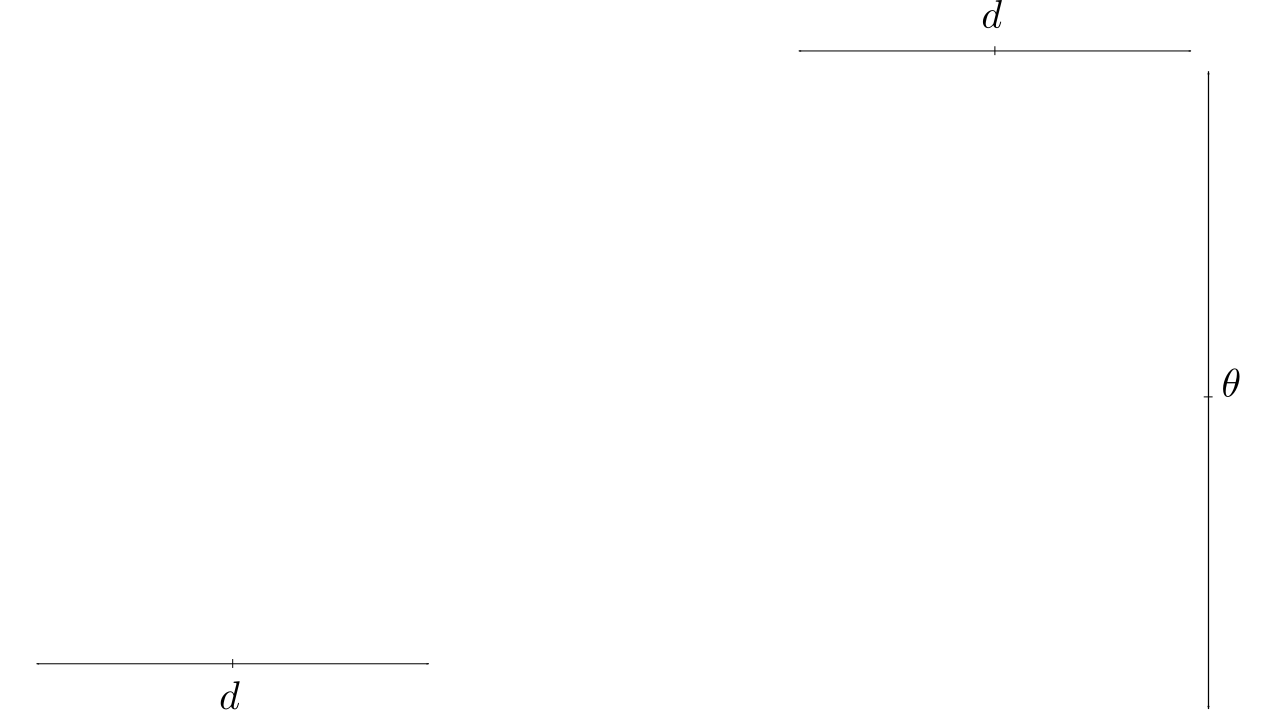
\includegraphics[width=11cm]{images/sino}
\caption[Principe du sinogramme]{Exemple de sinogramme: chaque ligne correspond à une projection de l'image selon un angle $\theta$ correspondant à la position de la ligne dans le sinogramme.}
\label{fig:sino}
\end{figure}











\chapter{Algorithmes de reconstruction}

La reconstruction des images TEP correspond à un problème inverse : à partir de l'ensemble des lignes de réponse, il faut déduire la répartition du radio traceur dans l'organisme du patient. Deux classes d'algorithmes existent pour résoudre ce type de problèmes, mais actuellement seuls les algorithmes itératifs sont utilisés en oncologie clinique. 

	\section{Algorithmes itératifs}

La relation liant l'image TEP $f$ et les projections sur les détecteurs $p$ est la suivante :

\begin{equation}
	p = R f + e
\label{eq:eqTEP}
\end{equation}

Avec $R$ la matrice de projection et $e$ correspondant aux phénomènes parasites. Ce problème est mal posé, car la perte d'information due aux projections ne garantit pas la résolution de ce problème. De plus, le bruit est un élément perturbateur supplémentaire. Il nécessite donc l'utilisation d'algorithmes spécialisés. 


		\subsection{Algorithme ML-EM (Maximum Likelihood Expectation Maximisation) }


L'algorithme ML-EM~\cite{shepp1982maximum} est initialisé avec une image de départ $f_0$, et considère que les comptages des lignes de réponses $p_i$ sont indépendants et bruités selon une loi de Poisson. Il se déroule en deux phases principales : une phase de comparaison de l'image au niveau $n$ avec les lignes de réponses observées, puis une phase de mise à jour de l'image pour prendre en compte les différences calculées à l'étape précédente, comme présenté dans la figure~\ref{fig:schemaMLEM}.

On considère les $(p_i)_{i=1..L}$, avec $L$ le nombre de projections, comme des variables aléatoires suivant une loi de Poisson dont la vraisemblance s'écrit :

\begin{equation}
proba(p|f) = \prod\limits_{i=1}^{L} \frac{<p_i>^{p_i}}{<p_i> !} e^{-<p_i>}
\label{lab:proba}
\end{equation}

Où $<p_i>$ est le paramètre de la loi de Poisson (moyenne) de la ligne de réponse $p_i$. L'objectif des algorithmes de reconstruction itératifs est d'estimer la distribution $f$ des $(f_j)_{i=j..P}$, avec $P$ le nombre de pixels, conduisant à l'ensemble $(<p_i>)_{i=1..L}$. L'équation~\ref{eq:eqTEP}, en négligeant les erreurs, s'écrit donc :

\begin{equation}
<p_i> = \sum\limits_{j=1}^{P} R_{ij}f_j
\end{equation}

On maximise la log-vraisemblance de l'équation~\ref{lab:proba} pour évaluer la cohérence entre les pixels de l'image $(f_j)_{j=1..P}$ et les projections observées $(p_i)_{i=1..L}$. Cette fonction de coût est notée $Q(f_1 \dots f_P, q_1 \dots q_L)$. On cherche l'estimation $\hat{f}$ de $f$ qui maximise cette fonction de coût :

\begin{equation}
	\hat{f}_j^{(n+1)}=\frac{\hat{f}_j^{(n)}}{\sum\limits_{i'}R_{i'j}}\sum\limits_{i}R_{ij}\frac{p_i}{\sum\limits_{k}R_{ik}\hat{f}_k^{(n)}}
\label{eq:MLEM}
\end{equation}

En pratique, la matrice système $R$ peut inclure des informations supplémentaires pour corriger les différences de sensibilité entre les différents capteurs, et réaliser la correction des diffusés~\cite{shepp1982maximum,chornoboy1990evaluation} ou la correction de l'atténuation des tissus. Cette matrice ``système'' $R_{ij}$ indique la probabilité de détecter une désintégration issue du voxel $j$ de l'image dans la ligne de réponse $i$.




Le nombre d'itérations à réaliser avant d'atteindre la convergence dépend de l'image, mais l'ordre de grandeur est d'environ 20 à 50. Il existe plusieurs publications proposant un critère d'arrêt~\cite{bissantz2006multi}, mais en pratique la reconstruction est souvent réalisée pour un nombre d'itérations élevées pour assurer la convergence~\cite{bailey2005positon} et  suivi d'un filtrage passe-bas~\cite{daube2001application} pour atténuer l'amplification du bruit. Cet algorithme de reconstruction prend un temps important car il faut réaliser l'opération de projection et de rétroprojection sur l'ensemble des données à chaque itération.

\begin{figure}
\centering
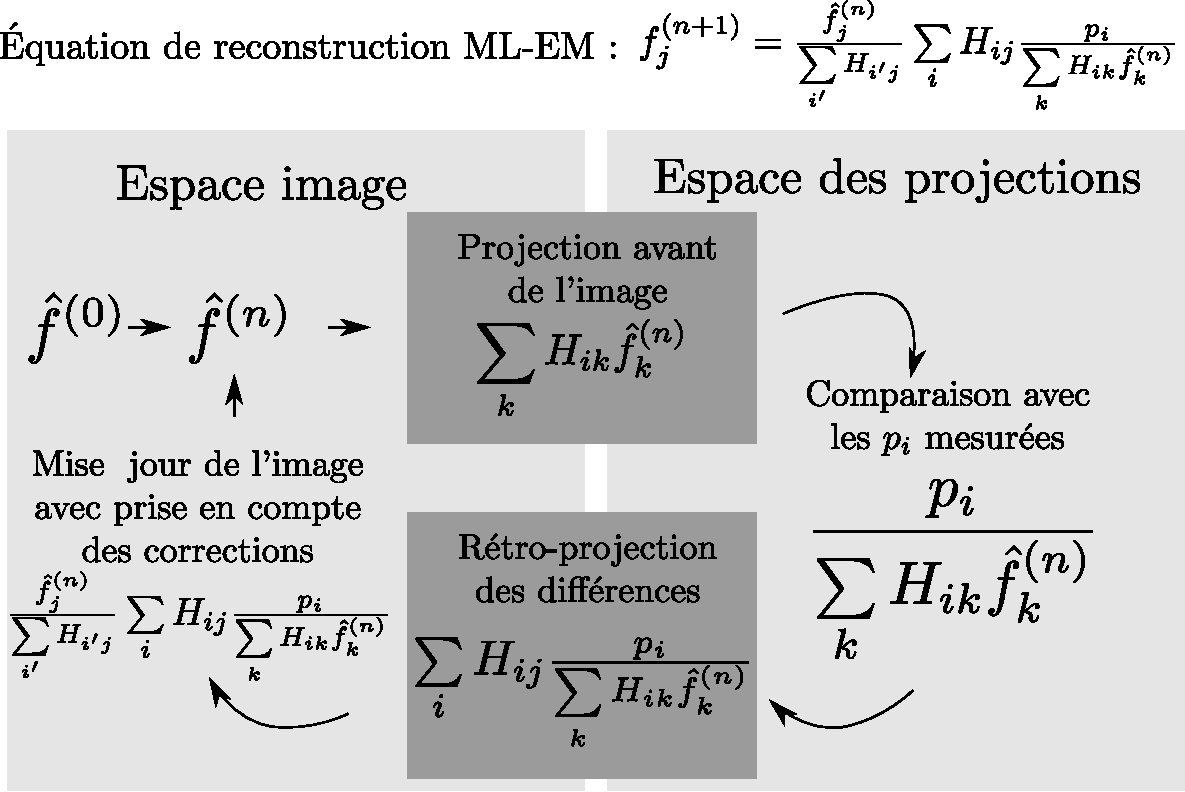
\includegraphics[width=12cm]{images/MLEM}
\caption[Schéma de principe de l'algorithme MLEM]{Schéma décrivant l'algorithme itératif ML-EM. $\hat{f}^{(n)}_j$ est l'estimation du voxel $j$ de l'image à l'itération $n$. $R_{ij}$ est la matrice système, et représente la probabilité de détecter une désintégration dans le voxel $j$ à la ligne de réponse $i$.}
\label{fig:schemaMLEM}
\end{figure}


	\subsection{Algorithme OS-EM (Ordered Subset Expectation Maximisation)}

L'algorithme OS-EM est une évolution de l'algorithme ML-EM  qui permet une accélération substantielle de la convergence en réalisant les itérations de l'équation~\ref{eq:MLEM} sur des sous-ensemble des données acquises~\cite{hudson1994accelerated}. 

Ces sous-ensembles de données sont réalisés en échantillonnant de manière régulière les lignes de réponses. Leur nombre est un des paramètres de l'algorithme, mais la convergence n'est plus garantie contrairement à ML-EM. En pratique, l'algorithme converge toujours approximativement, et le nombre d'itérations est déterminé de manière empirique~\cite{bailey2005positon}. Des évolutions de OS-EM ont été réalisées pour garantir une convergence, notamment l'algorithme Row-Action Maximum Likelihood (RAMLA)~\cite{browne1996row, chiang2004clinical}.

Le principal avantage de OS-EM est qu'il permet d'augmenter la vitesse de la reconstruction d'un facteur correspondant au nombre de sous-ensembles utilisés.

	\subsection{Cas des acquisitions en mode séquentiel}
\label{lab:OPLEM}

Les acquisitions en mode séquentiel génèrent une suite d'enregistrements correspondant aux événements détectés par l'imageur. La lecture de tous ces événements un par un demande des temps de calculs extrêmement importants, c'est pourquoi Reader et al.~\cite{reader2002one} ont proposé une adaptation de l'OS-EM au mode séquentiel appelée One-Pass List-Mode EM (OPL-EM). L'algorithme proposé est conçu pour ne parcourir qu'une seule fois la liste des événements. Comme pour OS-EM, les données sont groupées en sous-ensembles, qui sont utilisés les uns après les autres pour chaque itération, comme indiqué dans l'équation~\ref{eq:OSEM_seq}.

Ici, $s$ correspond à un numéro de sous-ensemble, $j$ à un voxel et $i$ à une ligne de réponse. Lorsque tous les sous-ensembles ont été parcourus, une nouvelle itération est déclenchée. Cet algorithme est conçu pour permettre de parcourir les données une seule fois, ce qui revient à réaliser une seule itération, cependant, il reste possible d'en réaliser plusieurs.

\begin{equation}
	f_j^{(s+1)}=\frac{\hat{f}_j^{(s)}}{\sum\limits_{i'}R_{i'j}}\sum\limits_{i \in T^s}R_{ij}\frac{1}{\sum\limits_{k}R_{ik}\hat{f}_k^{(s)}}
\label{eq:OSEM_seq}
\end{equation}

La différence entre OS-EM et cet algorithme est la manière dont sont sommées les différences. Dans OPL-EM, la sommation est réalisée sur l'ensemble des événements $T^s$ correspondant au sous-ensemble d'événements $s$. Cette somme est réalisée non pas pour chaque ligne de réponse $p$ comme précédemment, mais pour chaque événement détecté, ce qui explique le remplacement de $p_i$ par la valeur 1.
		
	\section{Reconstructions analytiques}

Ces algorithmes sont supplantés en oncologie par les algorithmes itératifs qui sont jugés plus performants sur l'évaluation du SUV et moins bruités~\cite{schoder2004clinical}.

Les méthodes analytiques utilisent la rétroprojection des projections du sinogramme pour reconstruire l'image. Si P est l'opération de projection d’une distribution $f(x,y)$ d’un objet vers $p(r, \theta)$, selon l’angle azimutal $\theta$, et $r$ la distance entre la projetée de la LDR dans le plan (x,y) et l’axe x, alors la projection peut s’écrire comme la transformée de Radon de cette distribution :
%\todo{revoir u et r}
\begin{equation}
p(u, \theta) = P(f(x,y)) = \int\limits_{-\infty}^{+\infty} f(u~cos \theta - v~cos \theta, u~sin \theta + v~cos \theta) dv
\end{equation}

avec la relation suivante entre $(x,y)$ et $(u,v)$ :

\begin{equation}
	\begin{bmatrix}
	x \\
	y
	\end{bmatrix}
	=	
	\begin{bmatrix}
	\cos \theta &  - \sin \theta \\
	\sin \theta & \cos \theta
	\end{bmatrix}
	\quad
	\begin{bmatrix}
	u \\
	v
	\end{bmatrix}
\end{equation}

L'opération de rétroprojection notée RP approxime l'opération inverse de la projection et permet d'obtenir l'estimation $\hat{f}(x,y)$ en fonction des projections acquises :

\begin{equation}
\hat{f}(x,y) = RP(p(u, \theta))
\end{equation}

La rétroprojection simple consiste à ajouter les contributions de chaque ligne de réponse à l'image estimée :

\begin{equation}
\hat{f}(x,y) = \int\limits_0^\pi p(u, \theta)d\theta
\label{eq:nonFiltree}
\end{equation}


Cependant cette rétroprojection génère des artefacts en ``étoile'' autour de l'objet. La rétroprojection filtrée~\cite{kinahan1988three} permet de limiter ces artefacts. Elle est basée sur le théorème de la coupe centrale pour réaliser la rétroprojection des données. Ce théorème démontre que la transformée de Fourier  monodimensionnelle de la projection $p(u,\theta)$ selon la direction $\theta$ est égale à la transformée bidimensionnelle de la distribution $f(x,y)$ selon un plan perpendiculaire à la direction de projection et passant par l'origine :

\begin{equation}
\left[ TF_{2D}(f) \right](\upsilon_x, \upsilon_y) = \left[ TF_{2D}(b) \right](\upsilon_x, \upsilon_y)|\upsilon|
\end{equation}

avec b(x,y) correspondant au résultat de la rétroprojection non filtrée de l'équation~\ref{eq:nonFiltree}. 

Les projections mesurées sont d'abord filtrées par le filtre rampe $\upsilon$ dans le domaine de Fourier. On rétroprojète ensuite la transformée de Fourier inverse de ces données filtrées. On obtient alors l'estimation de la distribution originale $\hat{f}$.